\documentclass{jdmdh}
\usepackage[utf8]{inputenc}
\usepackage{array}
\usepackage{pgfplots}
\usepackage{float}
\usepackage{tabularx}
\usepackage{titlesec}

\setcounter{secnumdepth}{3}
\pgfplotsset{compat=1.18}

\titlespacing*{\section}
{0pt}{2.5ex plus 1ex minus .2ex}{1.3ex plus .2ex}
\titlespacing*{\subsection}
{0pt}{1.0ex plus 1ex minus .2ex}{1.3ex plus .2ex}
\titlespacing*{\subsubsection}
{0pt}{1.0ex plus 1ex minus .2ex}{1.3ex plus .2ex}

\newcolumntype{C}{>{\arraybackslash}X} % centered "X" column


\title{You Actually Look Twice At it (YALTAi): using an object detection approach instead of region segmentation within the Kraken engine}
\author[1]{Thibault Clérice}
\affil[1]{Centre Jean-Mabillon, PSL Research University, France} 
\affil[2]{Hisoma (UMR 5189), Université Lyon 3, Université de Lyon (UDL), France} 

\corrauthor{Thibault Clérice}{thibault.clerice@chartes.psl.eu}


\begin{document}

\maketitle

\abstract{We did something awesome and wrote about it.}

\keywords{kraken;layout segmentation;yolo;htr;ocr;object detection;historical document}

\section{Introduction}

% Why the task you address is important, (if it is a new problem) problem statement, and applications
 
In recent years, automatic text extraction has become an important activity in digital philology and, in general, in corpus creation for historical documents. Few different engines share the software market: Transkribus and eScriptorium and its Kraken egnine are probably the two most known platforms. As model recognition improves over the year, the question of quasi-automatic corpus extraction from digitized manuscripts and early printed material has become more of a question of appropriate tooling rathen than HTR performances for specific fonts or languages and periods. On the side of Kraken, which has the advantage of being fully open-source, unlike Transkribus, the layout segmentation has suffered from poor performances perception by its users, specifically with small dataset (less than a thousand sample for train/eval/test) or very small dataset (less than 300 for train and val). 

This results perception has slowed the improvement of automatic information extraction, where the main body of text could be drawn from a printed book or a manuscript by ignoring marginal texts such as footnotes or running title. Extracting main body of works could result in creating data minable corpora of unprecedent sizes. We know of three research projects whose goals are hindered by the unability of Kraken to be trained with small dataset:

\begin{itemize}
    \item Pierre-Carl Langlais, Jean-Baptiste Camps, Nicolas Baumard and Olivier Morin's work on the evolution of French literary fictions from 1050 to the 1920s;
    \item Ariane Pinche's research project on medieval vernacular \textit{Légendiers}, compilations of Saint's Lives in Old French, with manuscripts split in multiple column;
    \item Simon Gabay and Béatrice Joyeux-Prunelle's work on manuscripts sales and art exhibition catalogs where the identification of each entry in the dataset leads to a lower amount of data to parse through natural language processing for denoising.
\end{itemize}

Historical document layout analysis has seen its first competition created in 2011 as a joint venture from the \textit{International Conference on Document Analysis and Recognition} (ICDAR2011) and the \textit{International Workshop on Historical Document Imaging and Processing} (HIP2011). The 2011 event limited itself to print document and tackled both the region segmentation operation as well as the region classification. In the context of ICDAR2011's Historical Document Layout Analysis competition (HDLA2011) and in general, layout segmentation is understood as the operation of recognizing blocks of content from the background in a digitized document. Region classification on the other hand is understood as the qualification of the blocks found during layout segmentation into various different categories. During ICDAR2011, document for the competition spanned from the 17\textsuperscript{th} to the early 20\textsuperscript{th} century and were segmented using polygons, which is the norm for this competition.

In 2011, methods for segmentation would mostly use a binarization step followed by some form of separator or content detection. 
ICDAR2017 had three relevant competitions:
\begin{itemize}
    \item the \textit{competition on Page Object Detection} (POD2017), whose dataset is composed of scientific papers in which the objective is to detect figures, tables, equations, etc.;
    \item the \textit{competition on Historical Book Analysis} (HBA2017), which has been renewed in 2019 (HBA2019);
    \item the \textit{competition on Layout Analysis for Challenging Medieval Manuscripts} (HisDoc-Layout-Comp).
\end{itemize}

While POD2017 sets the objective as a bounding box detection task, both HBA and HisDoc-Layout-Comp treats the task as a pixel labeling one, a pixel being able to be assigned to multiple task. Since 2017, deep learning models have emerged in the competition, specifically in HBA and HisDoc-Layout-Comp where CNN models shined. However, the shift from polygon detection at ICDAR2011 to pixel-based categorization at ICDAR 2019 creates a bias for the downstream task such as main body extraction: pixel categorization ignores the necessary serialization and clustering of said pixels into various zones that can then be filled with lines and content. This approach is specifically damageful in tools such as Kraken (v4.1.2) as it led to the creation of hacks, wich zones being qualified with \textit{ColumnEven} and \textit{ColumnOdd} systems in order to ensure the differentiation of columns in the clustering step.

With the specific purpose of training models on small datasets and document text extraction, we propose to approach the document segmentation as an object detection task, following the bounding box approach of ICDAR2017 instead of the polygon detection of ICDAR2011 or the pixel categorization of HBA or HisDoc-Layout-Comp. In this context, we propose two new datasets, a historical tabular document dataset (YALTAi-Tables) and a manuscripts and early printed book dataset (YALTAi-MSS-EPB). We do not propose a specific model but instead reuse 5\textsuperscript{th} version of You Only Look Once (YOLOv5)'s tools and models. Results show up to 100 times better results on column detection for tabular documents as well as doubles the score of main body document detection. As YOLOv5 base version is limited to ``straight'' boxes, it limits the application to lightly or unskewed documents. Bounding box can also overlap easily and we lose the precision of polygons.

\begin{figure}[ht]
    \centering
    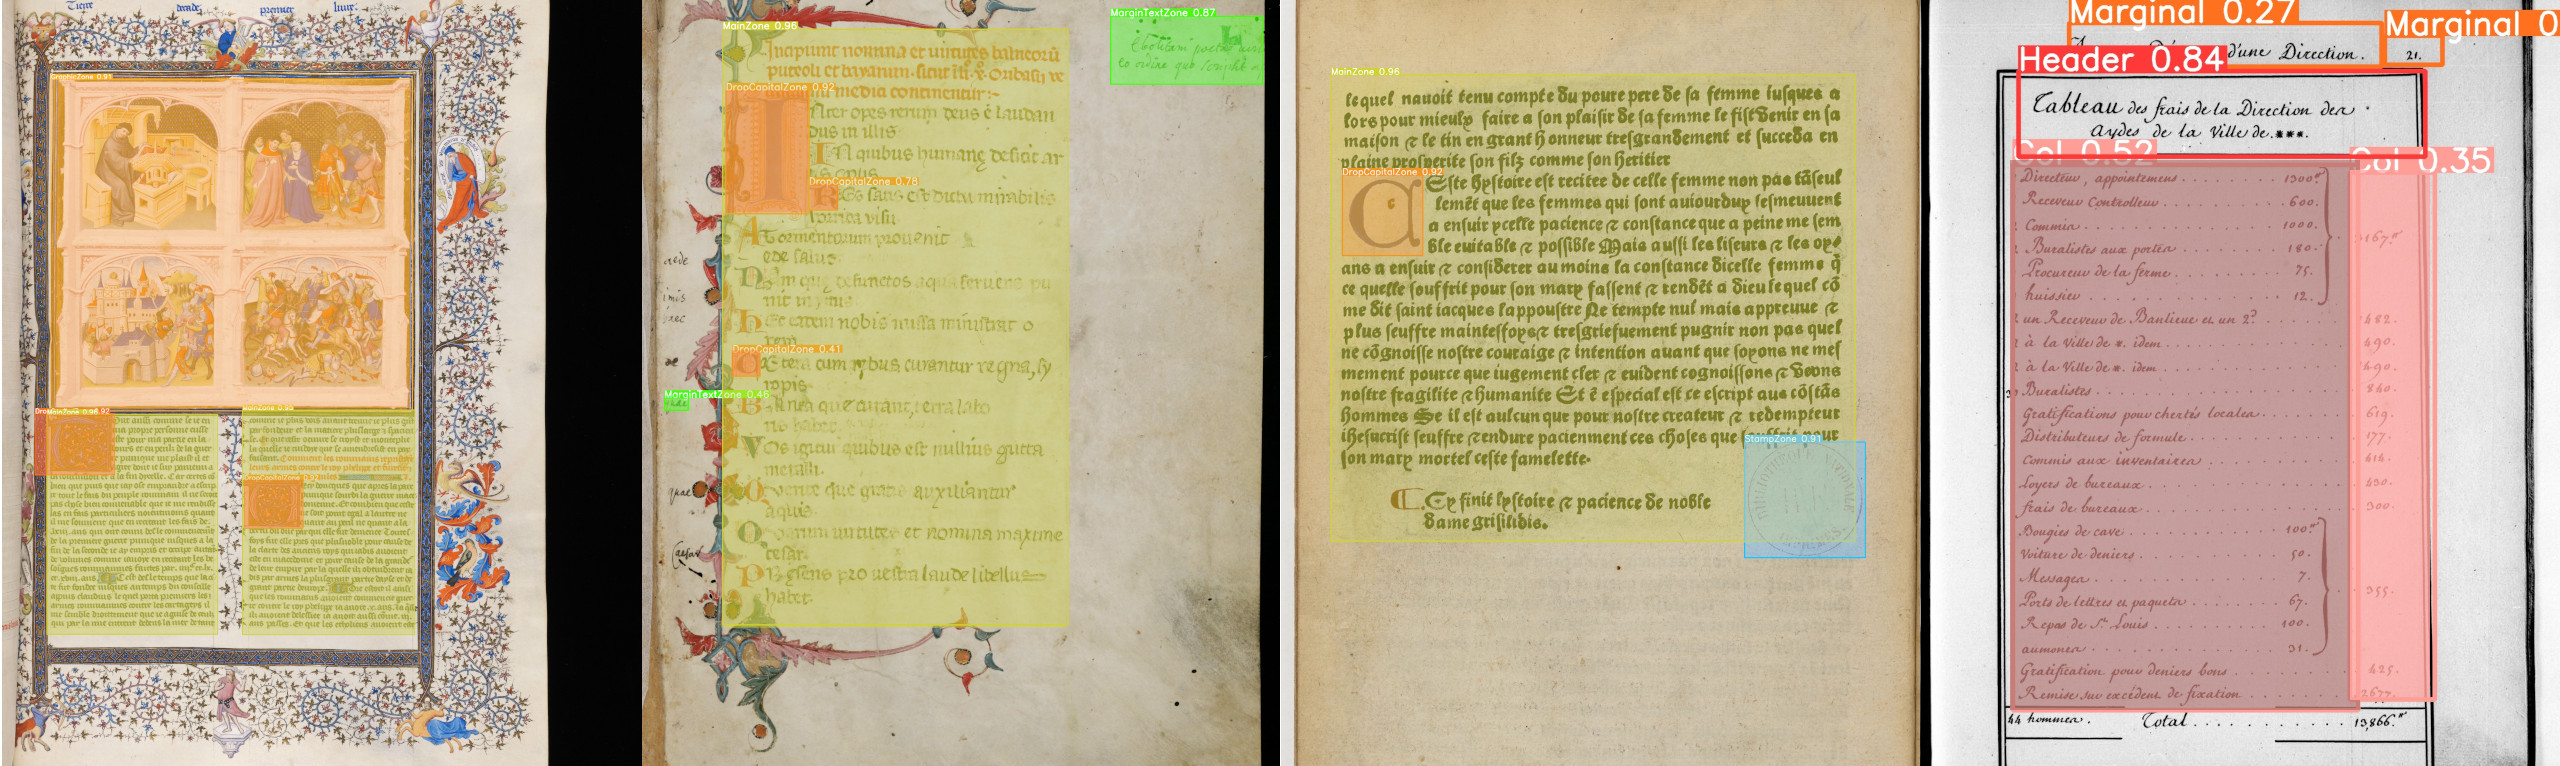
\includegraphics[width=\linewidth]{images/4images.jpg}
    \caption{Prediction on the test set with YOLOv5x models for the Segmonto dataset (three pictures on the left) and the tabular dataset (last picture, columns are in alternating colors for readability). Illustrations are in orange (first picture top), drop Capitals are in darker orange, marginal text in green, yellow is the main body of text.}
    \label{fig:4images}
\end{figure}

In summary, the contribution of this paper are:

\begin{enumerate}
    \item a proposal for shifting from polygon and pixel labeling to bounding box detection for documents that permits it at the layout detection stage;
    \item a new dataset for historical tabular document, spanning from the 16\textsuperscript{th} to the early 20\textsuperscript{th} century;
    \item a new dataset for the segmentation of historical documents such as manuscripts and early printed books (from the 9\textsuperscript{th} century to the 16\textsuperscript{16}) following the Segmonto ontology for segmentation classification labels;
    \item models for the detection of content regions according to both the Segmonto guidelines and a tabular approach;
    \item a tool, YALTAi, which allows for  \begin{itemize}
        \item the conversion of ALTO to YOLOv5 formats and vice-versa;
        \item accessing a command line interface similar to Kraken interface which injects the region detection of YOLOv5 at the time of line serialization for a seamlessly integration of the bounding box 
    \end{itemize}
\end{enumerate}

\section{Background and Related Work}
\label{sec:related}

\subsection{Background}

On a printed or manuscript page, conventions leads the organization of content on a page, such that element of a document can easily be processed by a human reader: a letter is usually formed of an opener, a body with one to many paragraphs, and a closer; a printed book usually contains a main body of texts -- be it paragraphs or lines and poems -- and a running title, a page number and optionally some margin information such as footnotes. Literary manuscripts follow such an organization, but are generally composed of two or more columns of main body of texts per page, each column is read from left to right so that when Column A is finished we start reading Column B. Such an organisation is crucial for the understanding of the content, as it allows the identification of contiguous blocks of main text and blocks of additional information for the human reader.

Segmonto provides a welcomed ontology and syntax for specifying the organization of pages from a layout perspective. \citet{gabay2021segmonto} define a serie of top level graphical structures that can be found in digitized document from medieval manuscripts up to comtemporaneous documents: main bodies of text are qualified as \texttt{MainZone}, marginal text such as footnotes and scribbles as \texttt{MarginZone}, paintings, photos and figures in general are represented by \texttt{GraphicZone} and specific medieval and modern early printed book features such as illuminated capitals fall under the category of \texttt{DropCapital}. These categorization can be refined at a second level with project-specific vocabulary which can contains categorization such as \texttt{MainZone:Entry} fr a dictionary entry or \texttt{MarginText:Footnote}. Documents automatically or manually tagged using this ontology allows for text extraction and data mining at scale without worrying with the noise of running titles or marginal text: preliminary work by \citet{christensen2022gallic} shows this possibility.

In his article ``Where is digital philology going''\footnote{French: ``Où va la philologie numérique ?''.}, \citet{camps2018o} analysed that Handwritten Text Recognition (HTR) can now be placed upstream of philological study, with downstream research taking advantage of the mass of data and multi-scale analysis for different tasks, from quantitative palaeography to computational stylistics. This inclusion of HTR in the workflow of medievalist and philologists in general has profited from the development of easy-to-use, highly available and performant HTR and OCR user interface. Research infrastructure software such as Transkribus \citep{kahle2017transkribus} or eScriptorium have taken their place in the humanist's office.

\citet{kiessling2019escriptorium} present Kraken and eScriptorium. Unlike Transkribus, it is built around fully installable and open-source practices, allowing for a take-and-go approach and not making the user prisoner within an ecosystem. Kraken is the computational software for training, evaluation and inference of models for both segmentation and text recognition tasks. Before eScriptorium, it could be used only through its python API or most likely with its command line interface (CLI). eScriptorium brought a user interface that allows for importing, segmenting, annotating and transcribing document, manually (no prediction provided by Kraken), semi-automatically (prediction provided and manually corrected) or automatically (prediction only).

\begin{figure}[h]
    \centering
    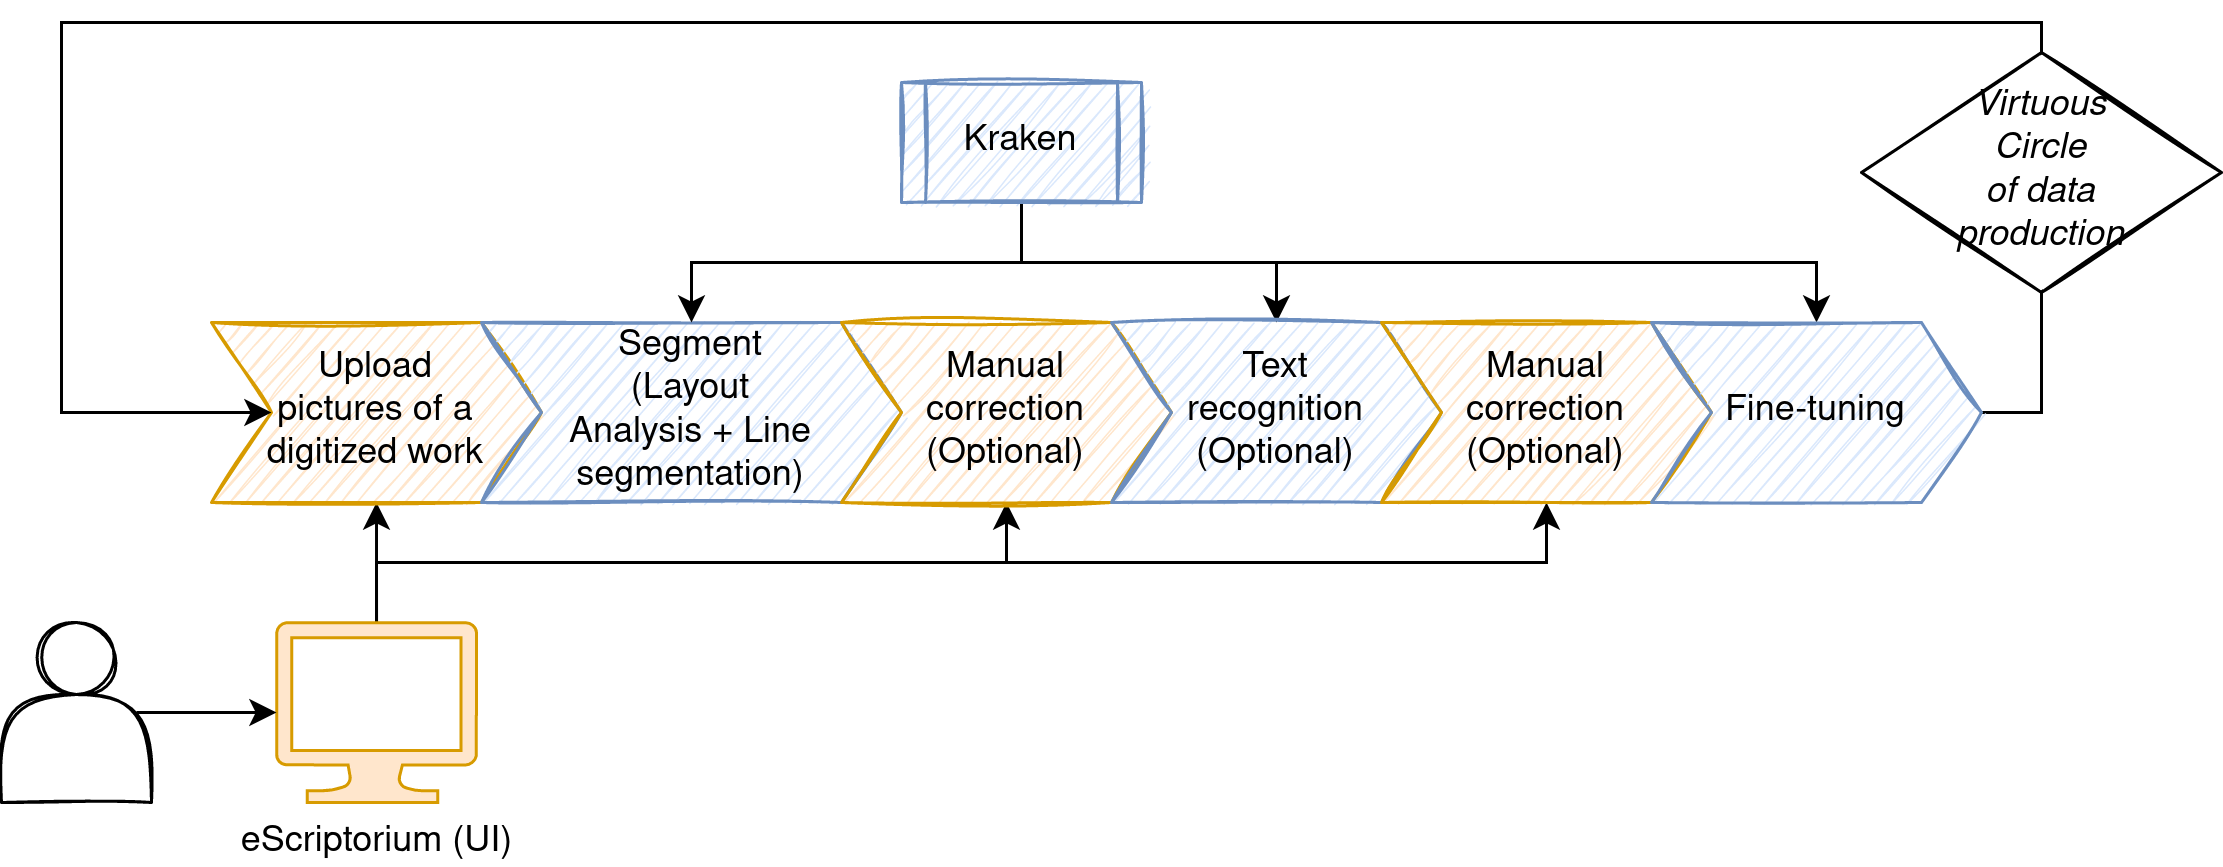
\includegraphics[width=\linewidth]{images/kraken-escriptorium.png}
    \caption{Typical Handwritten Text Recognition (HTR) workflow. A user uploads a set of pictures from a digitized book, segments the document both at the level of the layout and the lines, corrects the segmentation, provides a transcription or correct an automatic one and then fine-tune or creates models for other pages of the same document or documents of the same kind.}
    \label{fig:htr-workflow}
\end{figure}

\subsection{Related works}

In HDLA2011, \citet{antonacopoulos2011historical} defines layout analysis as both the action of identifying ``printed regions (Page segmentation) and labeling them according to the type of their content (Region Classification)''. Competitions of page segmentation have been run at ICDAR since 2001 and mostly on contemporary documents. 2011 was the first historical document oriented competition but restricted itself to printed material up to the 17\textsuperscript{th} century. In \citet{antonacopoulos2009icdar}'s review of ICDAR2009 Page Segmentation competition (PS2009), ground truth is defined by ``isothetic polygons (i.e. a polygon having only horizontal and vertical edges) [as] such a representation enables a very accurate and efficient geometric description, especially for complex-shaped regions''. 

In the late 2000s and the early 2010s, binarization and separator recognition, whether they are background separator (white space) or printed separator such as columns border, combined with different image analysis approach ruled the competitions. As of ICDAR2017, Convolutional Neural Networks and various other deep learning methods appeared in both HBA and HisDoc-Comp-Layout. However, \citet{antonacopoulos2009icdar} showed that non-deep learning methods could resist on complex document layout with DSPH getting the highest score of the competition: \citet{lu2021probabilistic} proposes a probabilistic approach to document segmentation and beats the first deep-learning based method of the competition by 15 points (95.1\% vs. 79.6\%).

In parallel with the development of layout analysis research, object detection research has made great strides from still image application to extending performance to real-time detection. Contrary to layout analysis, the object detection task aims at detecting so-called objects in pictures such as dogs, people or boats. It mainly operates with ``straight'' bounding box (with sides of the bounding box being only horizontal and vertical lines) but it also exists with oriented bounding box or masks. Unlike layout analysis, it deals with three dimensional information and as such different scales and different layers of information, from the foreground to the background. One of the main dataset for object detection model evaluation is the Microsoft COCO dataset and its evolutions. Described in \citet{lin2014microsoft}, COCO contains 91 kind of objects and 2.5 million instances accross 328,000 images.

In 2015, \textit{You Only Look Once} (YOLO) was released with its version 1 (YOLOv1). Each YOLO model has had in its core goals to detect quickly and close to real times instances of objects are at a high success rate. YOLOv1 used 24 convolution layers with two fully connected layers, splitting the picture into multiple cell and predicting for each cell what it could contain \citep{jiang2022a}. The use of YOLOv5 \citep{jocher2022ultralytics} in combination with OCR task is not novel, specifically for text transcription in scenes (\textit{e.g., }panels or license plate \citep{raj2022license}) or highly formatted documents such as receipts \citep{lin2022automatic}. Similarly to our work, \citet{ning2021mt} uses YOLOv5 on modern and contemporary documents for table detection but limits its work to table instances with scores on the lower end of the spectrum of state-of-the-art (SOTA) methods but with way fewer parameters (240M parameters for the best score vs. 7M for the implemented solution).

%We first review the literature on {relevant field}.
%Then, we focus on methods which {relevant approaches}, and {other related topic}

\section{Method}

We propose to shift the layout analysis task from a pixel categorization or polygon segmentation task to an object detection task, where each region is an instance of a category of zone, mixing the segmentation and classification part of the layout analysis. For the purpose of this paper, we work only with isothetic rectangles which are produced by using the minimal and maximal $X$ and $Y$ of each polygon, which results in a more important area captured by each zone. 

\begin{figure}
    \centering
    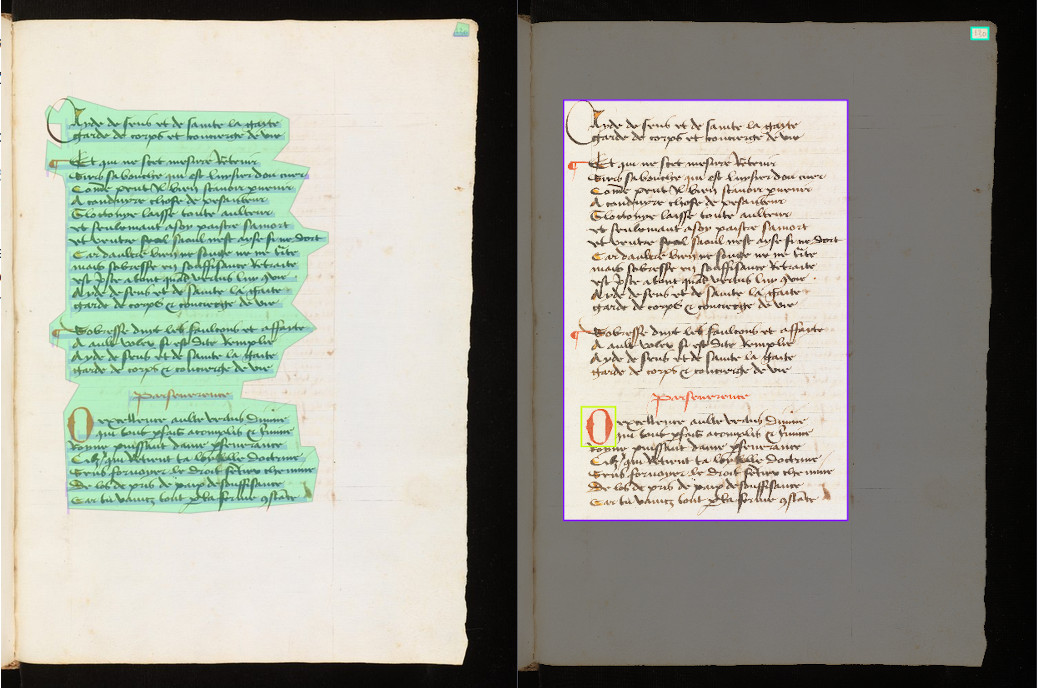
\includegraphics[width=.5\linewidth]{images/rectangulisation.jpg}
    \caption{Example of polygon in the ground truth when the Kraken prediction is correct on the left. On the right, its simplification into an isothetic rectangle for object detection.}
    \label{fig:yaltai:rectangulisation}
\end{figure}

In terms of software and model training, each model is kept independant: YoloV5 is trained within the YoloV5 framework and can profit from its ecosystem while Kraken line segmentation is also trained separately. Both model are then used together at inference or evaluation time.

As the objective is to provide end-users with a readily usable analysis of documents, the segmentation of zone should be fed in Kraken before the line detection is serialized, in order to dispatch lines into the various regions detected by YOLOv5. YOLOv5's output is serialized in the same fashion as Kraken region's segmentation output, such that it fits the expected input. Kraken uses the interpolation of the baseline to find the middle point and then uses the presence of the calculated point inside the region polygon to decide whether it belongs to the region (see Figure \ref{fig:yaltai:injection} for the details of the workflow at prediction time).

\begin{figure}
    \centering
    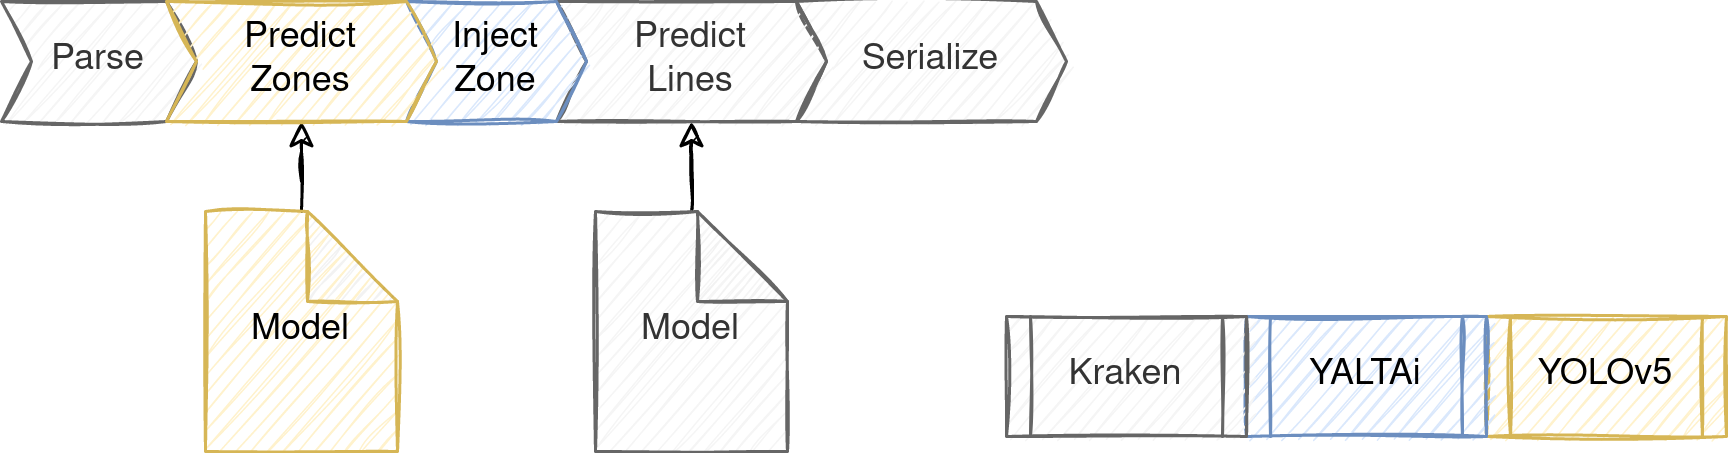
\includegraphics[width=.8\linewidth]{images/yaltaiinjection.png}
    \caption{Workflow and responsibilities at inference time.}
    \label{fig:yaltai:injection}
\end{figure}

\section{Experimental Setup}

The experimental setup is focused on evaluating the gains in terms of accuracy of zone detection or segmentation in historical document with ``complex'' layout. We compare YoloV5 models to Kraken segmentation model using the same datasets (described below) with fix split and using Mean Average Precision (mAP) as well as Average Precision (AP) for each class of categories that are relevant to the qualitative analysis of results.

\subsection{Datasets}

We built two datasets for the experiment and both Kraken and YOLOv5 are trained on the same rectangle-converted dataset. The first dataset consists of manuscripts and early printed book (YALTAi-MSS-EPB) from the 9\textsuperscript{th} century up to the 17\textsuperscript{th} century. It is based on five datasets:

\begin{itemize}
    \item CREMMA Medieval \citep{pinche2022cremma} focused on manuscripts in Old French with various layout and the inclusion of microfilm digitizations (Microfilm being black and white pictures).
    \item CREMMA Medieval LAT \citep{clerice2022cremma} contains manuscripts in Latin with different type of content, from poetry to medical content, which provides a diversity of layouts.
    \item Eutyches \citep{vlachou-efstathiou2022voss} focused on two manuscripts from the early Middle Ages.
    \item Two datasets from the Gallicorpora project (\citep{pinche2022donn, pinche2022donn2, pinche2022donn3}) containing either incunabilia, printed books with gothic scripts or manuscripts from the 15\textsuperscript{th} centuries, all writen in Old or Middle French.
\end{itemize}

On top of these five datasets, an addendum of 593 annotated images were produced for this paper to reach the objective of 1,000 images. This additional datasets provides a higher number of samples (123 different documents) and spans from the middle age to the early modern era (17\textsuperscript{th} century). These new annotated pages were produced with early version of the model and corrected by hand on the Roboflow application, thus they are more specific to the way YOLOv5 detects images and less prone to over-estimated area of polygon based on rectangle simplification as they are manually tuned to the images. The whole dataset uses Zone types from Segmonto, thus avoiding the project-specific and vocabulary free levels of subtypes and numbers that comes with Segmonto deeper levels.

\begin{table}[h]
    \centering
\resizebox{\linewidth}{!}{%}
    \begin{tabular}{l|rrrrrr}
         \hline
         Dataset & ``Books'' & Pages & Starting century & Ending century & Type & With B\&W \\ \hline
         \citep{pinche2022cremma} & 13 & 263 & 12 & 15 & Manuscripts & Yes \\
         \citep{clerice2022cremma} & 7 & 30 & 13 & 15 & Manuscripts & Yes \\ 
         \citep{vlachou-efstathiou2022voss} & 2 & 129 & 9 & 9 & Manuscripts & No \\
         \citep{pinche2022donn} & 4 & 80 & 15 & 15 & Printed & Yes \\
         \citep{pinche2022donn2} & 13 & 149 & 15 & 15 & Manuscripts & No \\
         \citep{pinche2022donn3} & 1 & 20 & 16 & 16 & Printed & No \\ \hline
         \textit{Original Data} & 123 & 593 & 9 & 17 & Printed & No \\ \hline
    \end{tabular}%
    }
    \caption{Quantitative and qualitative description of YALTAi MSS EPB. ``Books'' can be full manuscripts or printed books. \textit{Original data} are previously unpublished data produced directly using bounding boxes.}
    \label{tab:dataset:mssepb}
\end{table}

\section{Experiments}



\begin{table}[]
\resizebox{\linewidth}{!}{%}
\begin{tabular}{l|r|rrrrrrrrr}
\hline
        & mAP            & Main          & Graphic        & DropCapital     & MarginText     & Numbering      & QuireMarks     & RunningTitle   & Stamp        \\ \hline
Kraken  & 6.98           & 43.5          & 16.1           & 23.3            & 0.0            & 0.0            & 0              & 0              & 0            \\
YoloV5x & \textbf{47.75} & \textbf{91.7} & \textbf{48.4}  & \textbf{69.2}   &  \textbf{48.3} &  \textbf{75.8} & \textbf{46.3}  &          45.6  & \textbf{100} \\ 
YoloV5n &         34.63  &        87.0   &         44.2   &         54.6    &         13.9   &         43.0   &         25.0   &  \textbf{48.1} & \textbf{100} \\ \hline
\end{tabular}%
}
\label{tab:scores:segmonto}
\caption{Scores of Kraken and YoloV5 best models for the Segmonto MSS and Early Printed Books Dataset. Zones (Main, Graphic, Drop Capital, Margin Text, Numbering, Quire Marks, Running Title and Stamp) are the most important zones from the test dataset. Scores for zones are the Average Precision. Both Mean Average Precision and Average Precision are given in percents. Surprisingly, YoloV5n beats YoloV5x on RunningTitle but is most often largely outperformed on other zones. Kraken is completely outperformed with YoloV5x more than doubling its scores on the main body zones, and roughly multiplying it by 7 times for the mean average precision.}
\end{table}

\begin{table}[]
\begin{center}
\begin{tabular}{l|r|rrrr}
\hline
        & mAP           & Col           & Header       & Marginal \\ \hline
Kraken  & 0.09          & 0.1           & 0.1          & N/A      \\
YoloV5x & \textbf{4.77} & \textbf{12.9} & \textbf{1.4} & 0        \\  \hline       
\end{tabular}
\end{center}
\label{tab:scores:table}
\caption{Scores of Kraken and YoloV5 best models for the Table Dataset. \textit{Col}, \textit{Header} and \textit{Marginal} are the three detected kind of zones. Scores for zones are the Average Precision. Both Mean Average Precision and Average Precision are given in percents. The YoloV5x performs a hundred time better than Kraken on Columns while it has a 53 times higher mean Average Precision.}
\end{table}


\begin{table}[]
\resizebox{\linewidth}{!}{%}
\begin{tabular}{l|rrrrrrrr}
\hline
       & Dataset  & Batch Size & Architecture & Size            & GPU Power (Max)   & GPU RAM \% (Max)   & Training Time & Prediction Time \\ \hline
Kraken & Table    & 1          & 640          & \textbf{5 mb}   & 202.1 W           & \textbf{25.44 \%}  &  00:50        &                 \\
YoloV5 & Table    & 2          & 5x           & 175 mb          & \textbf{157.2 W}  & 67.85              &  00:25        &                 \\\hline
Kraken & Segmonto & 1          & 1200         &         5 mb    & 236.1 W           & 66.02 \%           &  06:27        &                 \\
YoloV5 & Segmonto & 2          & 5x           & 175 mb          & 160.43 W          & 39.31 \%           &  03:04        & 0.025s          \\
YoloV5 & Segmonto & 2          & 5n           & \textbf{3.9 mb} & \textbf{54.05 W}  & \textbf{11.5 \%}   &  03:11        & 0.004s          \\ \hline
\end{tabular}%\
}
\label{tab:scores:configs}
\caption{Other metrics related to Kraken and YoloV5. YoloV5x produces the heaviest model (175mb, 35 times the weight of the Kraken model) but uses at most 77\% of the maximum power draw of Kraken. Training time is generally doubled under Kraken. For the segmonto model, the maximum GPU RAM usage is halved for YoloV5N, while using a batch of 2, but is nearly three times the footprint of Kraken for the Table dataset.}
\end{table}

\section{Conclusions}

\subsection{Acknowledgements}

\bibliographystyle{plainnat}
\bibliography{article}

\end{document}